\label{appendix:eds_images}

This appendix presents the complete collection of EDS images for all analyzed spots across different Si/Al ratios.
All specimens were cured for 3 days at 60°C and 1000× magnification.

For each Si/Al ratio, atomic and weight percentages spectrums are provided, together with EDS layered images and corresponding EDS maps for the analyzed spots.

\section{Si/Al = 0.9}

\begin{table}[H]
    \centering
    \caption{EDS spectrum of Si/Al = 0.9 pastes after 3 days of curing at 60$\degree$C.}
    \label{tab:eds_spectrum_0-9}
    \begin{tabular}{l c c c c c c c c}
        \hline
        \multicolumn{1}{c}{Sample} & \multicolumn{4}{c}{At(\%)} & \multicolumn{4}{c}{Wt(\%)} \\
        \cline{2-9}
        & Si & Al & K & Ca & Si & Al & K & Ca \\
        \hline
        0.9\textunderscore 60C\textunderscore 3d\textunderscore Spot1  &   &   &   &   &   &   &   &  \\
        0.9\textunderscore 60C\textunderscore 3d\textunderscore Spot2  &   &   &   &   &   &   &   &  \\
        0.9\textunderscore 60C\textunderscore 3d\textunderscore Spot3  &   &   &   &   &   &   &   &  \\
        0.9\textunderscore 60C\textunderscore 3d\textunderscore Spot4  &   &   &   &   &   &   &   &  \\
        0.9\textunderscore 60C\textunderscore 3d\textunderscore Spot5 & 26.4 & 27.1 & 30.4 & 16.0 & 22.4 & 22.1 & 36.0 & 19.5 \\
        0.9\textunderscore 60C\textunderscore 3d\textunderscore Spot6  &   &   &   &   &   &   &   &  \\
        \hline
    \end{tabular}
\end{table}

\section{Si/Al = 3.0}

\begin{table}[H]
    \centering
    \caption{EDS spectrum of Si/Al = 3.0 pastes after 3 days of curing at 60$\degree$C.}
    \label{tab:eds_spectrum_3-0}
    \begin{tabular}{l c c c c c c c c}
        \hline
        \multicolumn{1}{c}{Sample} & \multicolumn{4}{c}{At(\%)} & \multicolumn{4}{c}{Wt(\%)} \\
        \cline{2-9}
        & Si & Al & K & Ca & Si & Al & K & Ca \\
        \hline
        3.0\textunderscore 60C\textunderscore 3d\textunderscore Spot1  &   &   &   &   &   &   &   &  \\
        3.0\textunderscore 60C\textunderscore 3d\textunderscore Spot2  &   &   &   &   &   &   &   &  \\
        3.0\textunderscore 60C\textunderscore 3d\textunderscore Spot3 & 54.2 & 13.5 & 21.5 & 10.8 & 48.2 & 11.5 & 26.6 & 13.7 \\
        3.0\textunderscore 60C\textunderscore 3d\textunderscore Spot4  &   &   &   &   &   &   &   &  \\
        3.0\textunderscore 60C\textunderscore 3d\textunderscore Spot5  &   &   &   &   &   &   &   &  \\
        3.0\textunderscore 60C\textunderscore 3d\textunderscore Spot6  &   &   &   &   &   &   &   &  \\
        \hline
    \end{tabular}
\end{table}

\section{Si/Al = 5.0}

\begin{table}[H]
    \centering
    \caption{EDS spectrum of Si/Al = 5.0 pastes after 3 days of curing at 60$\degree$C.}
    \label{tab:eds_spectrum_5-0}
    \begin{tabular}{l c c c c c c c c}
        \hline
        \multicolumn{1}{c}{Sample} & \multicolumn{4}{c}{At(\%)} & \multicolumn{4}{c}{Wt(\%)} \\
        \cline{2-9}
        & Si & Al & K & Ca & Si & Al & K & Ca \\
        \hline
        5.0\textunderscore 60C\textunderscore 3d\textunderscore Spot1 & 59.5 & 9.2 & 19.6 & 11.6 & 53.0 & 7.9 & 24.2 & 14.9 \\
        5.0\textunderscore 60C\textunderscore 3d\textunderscore Spot2  &   &   &   &   &   &   &   &  \\
        5.0\textunderscore 60C\textunderscore 3d\textunderscore Spot3  &   &   &   &   &   &   &   &  \\
        5.0\textunderscore 60C\textunderscore 3d\textunderscore Spot4  &   &   &   &   &   &   &   &  \\
        5.0\textunderscore 60C\textunderscore 3d\textunderscore Spot5  &   &   &   &   &   &   &   &  \\
        5.0\textunderscore 60C\textunderscore 3d\textunderscore Spot6  &   &   &   &   &   &   &   &  \\
        \hline
    \end{tabular}
\end{table}

\begin{figure}[H]
    \centering
    \subfloat[EDS layered image]{
        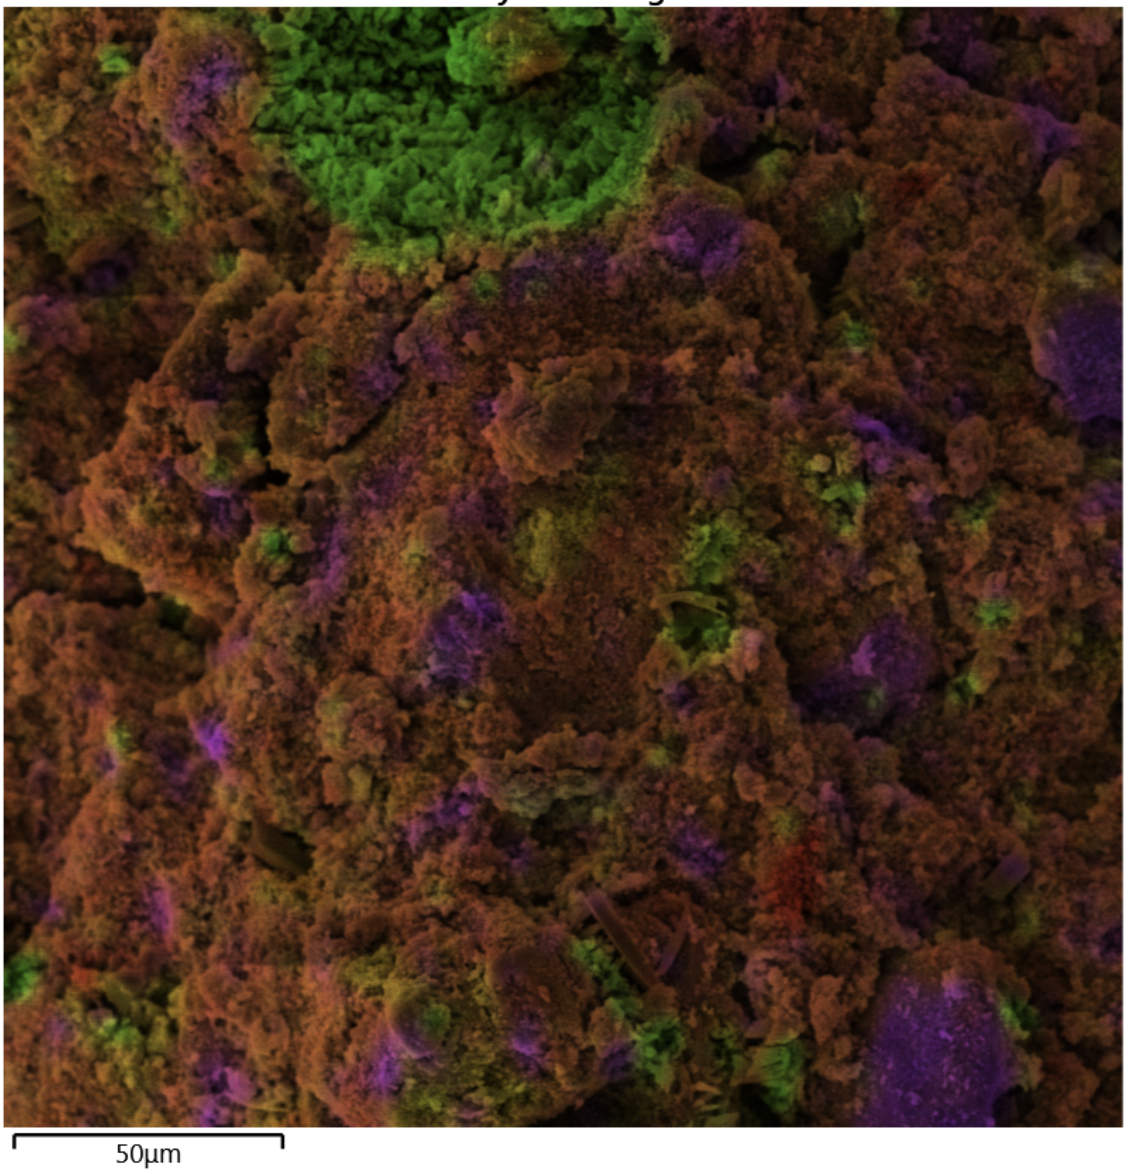
\includegraphics[height=6cm]{AppendixC/images/5-0-60C-3d-Spot 1 - layered.png}
    }
    \hfill
    \subfloat[EDS map]{
        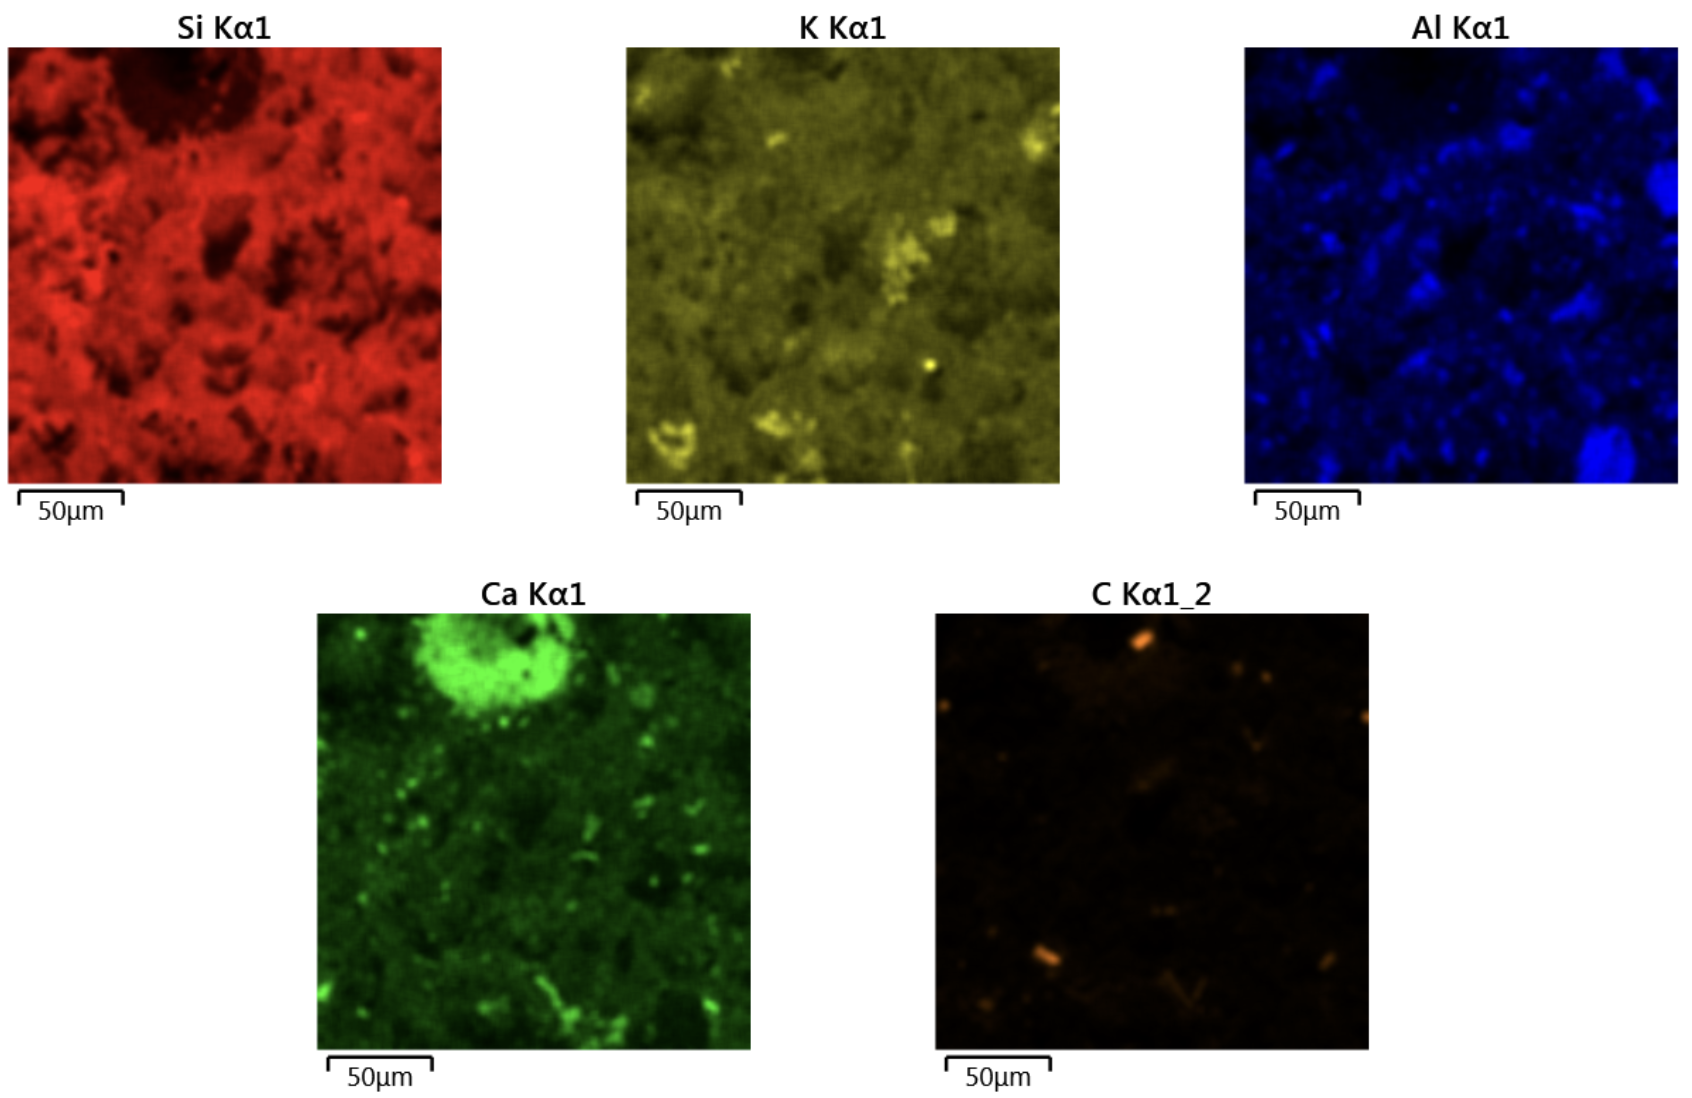
\includegraphics[height=6cm]{AppendixC/images/5-0-60C-3d-Spot 1 - map.png}
    }
    \caption{EDS analysis of Spot 1, Si/Al = 5.0, cured for 3 days at 60°C at 1000× magnification.}
    \label{fig:eds_spot1_5-0}
\end{figure}

